\documentclass[12pt,a4paper]{article}

\usepackage[UTF8]{ctex}
\usepackage{amsmath,amscd,amsbsy,amssymb,latexsym,url,bm,amsthm}
\usepackage{amsfonts}
\usepackage{epsfig,graphicx,subfigure}
\usepackage{hyperref}
\usepackage{listings}
\usepackage[vlined,ruled,linesnumbered]{algorithm2e}
\usepackage{enumitem}
\usepackage{xcolor}
\usepackage{geometry}

%\uppercase\expandafter{\romannumeral1}:% 罗马数字。

\lstset{
language=Matlab,
keywordstyle= \color{blue!70},
commentstyle= \color{red!50!green!50!blue!50},
breaklines
}%设置listing插入语言

\setlength{\parindent}{0em}
\setlength{\parskip}{1em}

\geometry{bottom =3cm}
\newcommand{\textbi}[1]{%
\textbf{\textit{#1}}}

\newcommand{\ncolor}[1]{%
{\color[RGB]{139,117,0}{#1}}}
\newtheorem{theorem}{Theorem}[section]
\newenvironment{solution}{{\noindent \it \textbf{Solution:}}\\}

\title{Queuing Theory and Random Process}
\author{Yunlong Cheng}

\begin{document}
\maketitle
\section{概念}
\subsection{随机过程}
一组随机变量,即指定一组参数集,对于其中每一参数点指定一个随机变量 $x(t)$,以 $\omega$ 表示随机变量 $x(t)$ 的定义域中的一点,则点偶 $(t,\omega)$ 以及概率分布完全确定随机过程。
\subsection{计数过程}
$\{N(t),t\ge 0\}$
\begin{itemize}
  \item 对$t_1<t_2$,有$N(t_1)\le N(t_2)$
  \item 对$t_1<t_2$,$N(t_2) - N(t_1)$ 为时间间隔 $[t_1,t_2]$ 之间发生的事件总数。
\end{itemize}

\subsection{独立增量和平稳增量}
\subsection{泊松过程}
是最重要的计数过程。
满足长度为 $t$ 的任意时间区间的时间个数服从均值为 $\lambda t$ 的泊松分布。
$$P\{N(s+t) - N(s) = n\} = e^{-\lambda t}\frac{{(\lambda t)}^n}{n!}$$
{\color{red} 重要性质和概念:}
\begin{itemize}
  \item $E\{N(t)\} = \lambda t\quad\lambda $称为泊松过程的速率
  \item $P(\text{两次事件之间的间隔}) = e^{-\lambda t}$
\end{itemize}
\subsection{排队论肯德尔记号}
X/Y/Z/A/B/C :
\begin{itemize}
  \item X - 顾客相继到达的间隔时间的分布。
  \item Y - 服务时间的分布。

  X,Y的取值可以为:M - 指数分布,G - 一般分布
  \item Z - 服务台个数。
  \item A - 系统容量限制,默认为$\infty$
  \item B - 顾客源数目,默认为$\infty$
  \item C - 服务规则,默认为 $FCFS$
\end{itemize}
\subsection{排队论基本量和价格方程}
\begin{itemize}
  \item L - 系统中顾客平均数。
  \item $L_Q$ - 队列中平均等待顾客数。
  \item W - 一个顾客在系统中所耗的平均时间。
  \item $W_Q$ - 一个顾客在队列中等待的平均时间。
  \item 系统赚钱的平均速率 = $\lambda_a\times$ 进入系统的顾客所支付的平均金额

  其中 $\lambda_a = \lim_{t\to \infty}\frac{N(t)}{t}$
\end{itemize}
三个规则(对所有价格方程都成立,由 Little 公式保证):
\begin{itemize}
  \item $L = \lambda_a\times W$
  \item $L_Q = \lambda_a\times W_Q$
  \item $1 - P_0 = \lambda_a\times E(S)$
\end{itemize}
\subsection{稳态概率}
系统中有 n 个顾客的长程概率 $P_n = \lim_{t\to \infty}P\{X(t) = n\}$,$P_0$ 表示系统处于空闲的概率。
\subsection{平衡方程}
进入状态 n 的速率 = 离开状态 n 的速率
\begin{center}
  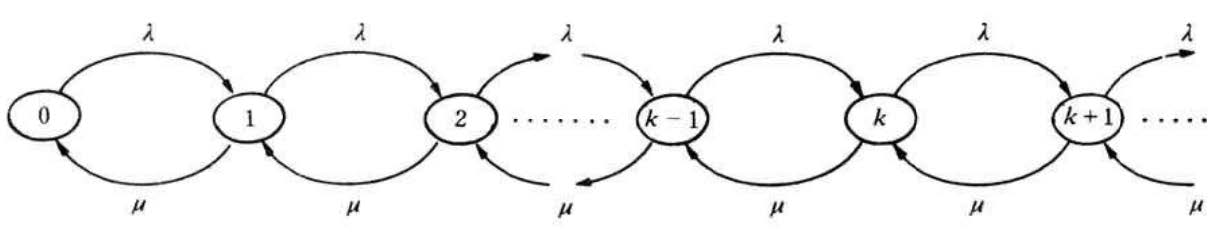
\includegraphics[width  = \textwidth]{figures/stable_equation}
\end{center}
$\lambda,\mu$ 为顾客进入/离开平均速率

\section{模型}
\subsection{M/M/1型}
\begin{enumerate}
  \item 平衡方程与约束条件:
  \begin{center}
    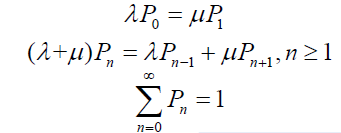
\includegraphics[width  = 0.6\textwidth]{figures/MM1}
  \end{center}
  \item 性能指标计算:
  \begin{equation*}
    \begin{split}
      L & = \frac{\lambda}{\mu - \lambda}\\
      W & = \frac{L}{\lambda} = \frac{1}{\mu - \lambda}\\
      W_Q & = W - E(s) = \frac{\lambda}{\mu(\mu - \lambda)}\\
      & E(S) = \frac{1}{\mu}\;\text{为一个顾客被服务的平均时间}\\
      L_Q & = \lambda W_Q = \frac{\lambda^2}{\mu(\mu - \lambda)}\\
    \end{split}
  \end{equation*}
\end{enumerate}

\subsection{有限容量的M/M/1型(变形1)}
因为是有限容量所以存在最后一个状态。

最后一个平衡方程:
$$\mu P_N = \lambda P_{N - 1}$$
性能指标:
$$W = \frac{L}{\lambda_a}$$
$$\lambda_a = \lambda(1 - P_n)$$
\subsection{到达率和离开率不是定值(变形2)}
\subsection{M/M/k型(变形三)}
$$\lambda_n = \lambda$$
\begin{equation*}
  \mu_n =
  \begin{cases}
    n\mu & n < k\\
    k\mu & n \ge k\\
  \end{cases}
\end{equation*}

\section{排队论分析思路}
\begin{enumerate}
  \item 分析系统状态空间及转换关系.
  \item 根据转换关系列出平衡方程.
  \item 求解平衡方程(逐差法、观察法).
  \item 计算性能指标(级数求和、价格方程)
\end{enumerate}

\end{document}
